\section{Χαρακτηριστικά που υλοποιήθηκαν} \label{section:4-5-implemented-parts}

Κατά την υλοποίηση εμφανίστηκαν διάφορα προβλήματα που δεν είχαν προβλεφθεί όπως αναλύθηκε στο προηγούμενο κεφάλαιο και τα οποία προκάλεσαν καθυστερήσεις στην ολοκλήρωση των tasks. Λόγω των καθυστερήσεων αυτών έγιναν διάφορες αναδιαμορφώσεις του προγραμματισμού των Sprint καθώς και διαπραγματεύσεις της σημαντικότητας των χαρακτηριστικών. Από τον επανασχεδιασμό και τις προσαρμογές αυτές προέκυψαν μερικές αλλαγές στο τελικό σετ των χαρακτηριστικών της πλατφόρμας σε σχέση με ό,τι είχε αρχικά προδιαγραφεί. Τα χαρακτηριστικά που υλοποιήθηκαν είναι:

\begin{itemize}
    \item η εγγραφή χρήστη (\ref{subsection:3-6-use-case-signup})
    \item η αυτόματη είσοδος χρήστη (\ref{subsection:3-6-use-case-signin})
    \item η δημιουργία θέματος (\ref{subsection:3-6-use-case-create-topic})
    \item η περιήγηση στα υπάρχοντας θέματα (\ref{subsection:3-6-use-case-fetch-topic})
    \item η δημοσίευση μηνύματος (\ref{subsection:3-6-use-case-create-post})
    \item η επεξεργασία μηνύματος (\ref{subsection:3-6-use-case-modify-post})
    \item η ψήφιση σε ψηφοφορία (\ref{subsection:3-6-use-case-vote-in-poll})
    \item η ψήφιση σε μηνύματα (\ref{subsection:3-6-use-case-vote-post})
    \item η διαγραφή των τοπικών δεδομένων (\ref{subsection:3-6-use-case-delete-local-data})
\end{itemize}

Στο παράρτημα \ref{screenshots-appendix} παρατίθενται τα στιγμιότυπα οθόνης των υλοποιημένων χαρακτηριστικών.

Τα χαρακτηριστικά τα οποία παραλήφθηκαν είναι τα παρακάτω:
% TODO: fix item names here and add refs to the actual use cases once they are created

\begin{itemize}
    \item serve (front and contracts) thru IPFS
    \item upgradability
\end{itemize}

\subsection{Διαφορές σχεδιασμού-υλοποίησης} \label{subsection:4-6-1-design-implementation-differences}

Σημαντικές διαφορές υπήρξαν επίσης στην διαδικασία υλοποίησης τόσο όσον αφορά τον αριθμό και τις λειτουργίες των διαφορετικών πακέτων λογισμικού όσο και τον χρονοπρογραμματισμό. Προστέθηκαν τρεις νέες υπηρεσίες, η υπηρεσία "Concordia Contracts Provider", ο προσαρμοσμένος IPFS pinner και η ιστοσελίδα "Concordia Guide".

Η ανάγκη για τα νέα πακέτα λογισμικού προέκυψε κατά την πορεία υλοποίησης της διπλωματικής και προστέθηκαν στον χρονοπρογραμματισμό που είχε γίνει στην αρχή της εργασίας. Στην προσαρμογή αυτή βοήθησαν ιδιαίτερα οι Agile τακτικές που ακολουθήθηκαν και η προσαρμοστικότητα που προσφέρει το Scrum σε μεταβαλλόμενες απαιτήσεις.

Τέλος, κατά την υλοποίηση έγινε γρήγορα αντιληπτή η αξία που προσφέρουν ένα δοκιμαστικό περιβάλλον (staging environment) σε συνδυασμό με ένα CI/CD σύστημα. Για το λόγο αυτό πάρθηκε η απόφαση να μεταφερθεί το sprint που αφορούσε αυτά πολύ νωρίτερα στην διαδικασία υλοποίησης, ώστε να μεγιστοποιηθεί η χρήση του.

Εποπτικά, η διαδικασία της υλοποίησης περιγράφεται στο παρακάτω σχήμα (σχήμα \ref{figure:4.6.design-implementation-differences-sprints}). Με σκούρο πράσινο χρώμα εμφανίζονται τα tasks τα οποία υπήρχαν στο χρονοπρογραμματισμό από τη αρχή και υλοποιήθηκαν, με ανοιχτό πράσινο αυτά τα οποία δεν υπήρχαν στον αρχικό προγραμματισμό αλλά υλοποιήθηκαν και με κόκκινο αυτά τα οποία δεν υλοποιήθηκαν.

\begin{figure}[H]
    \centering
    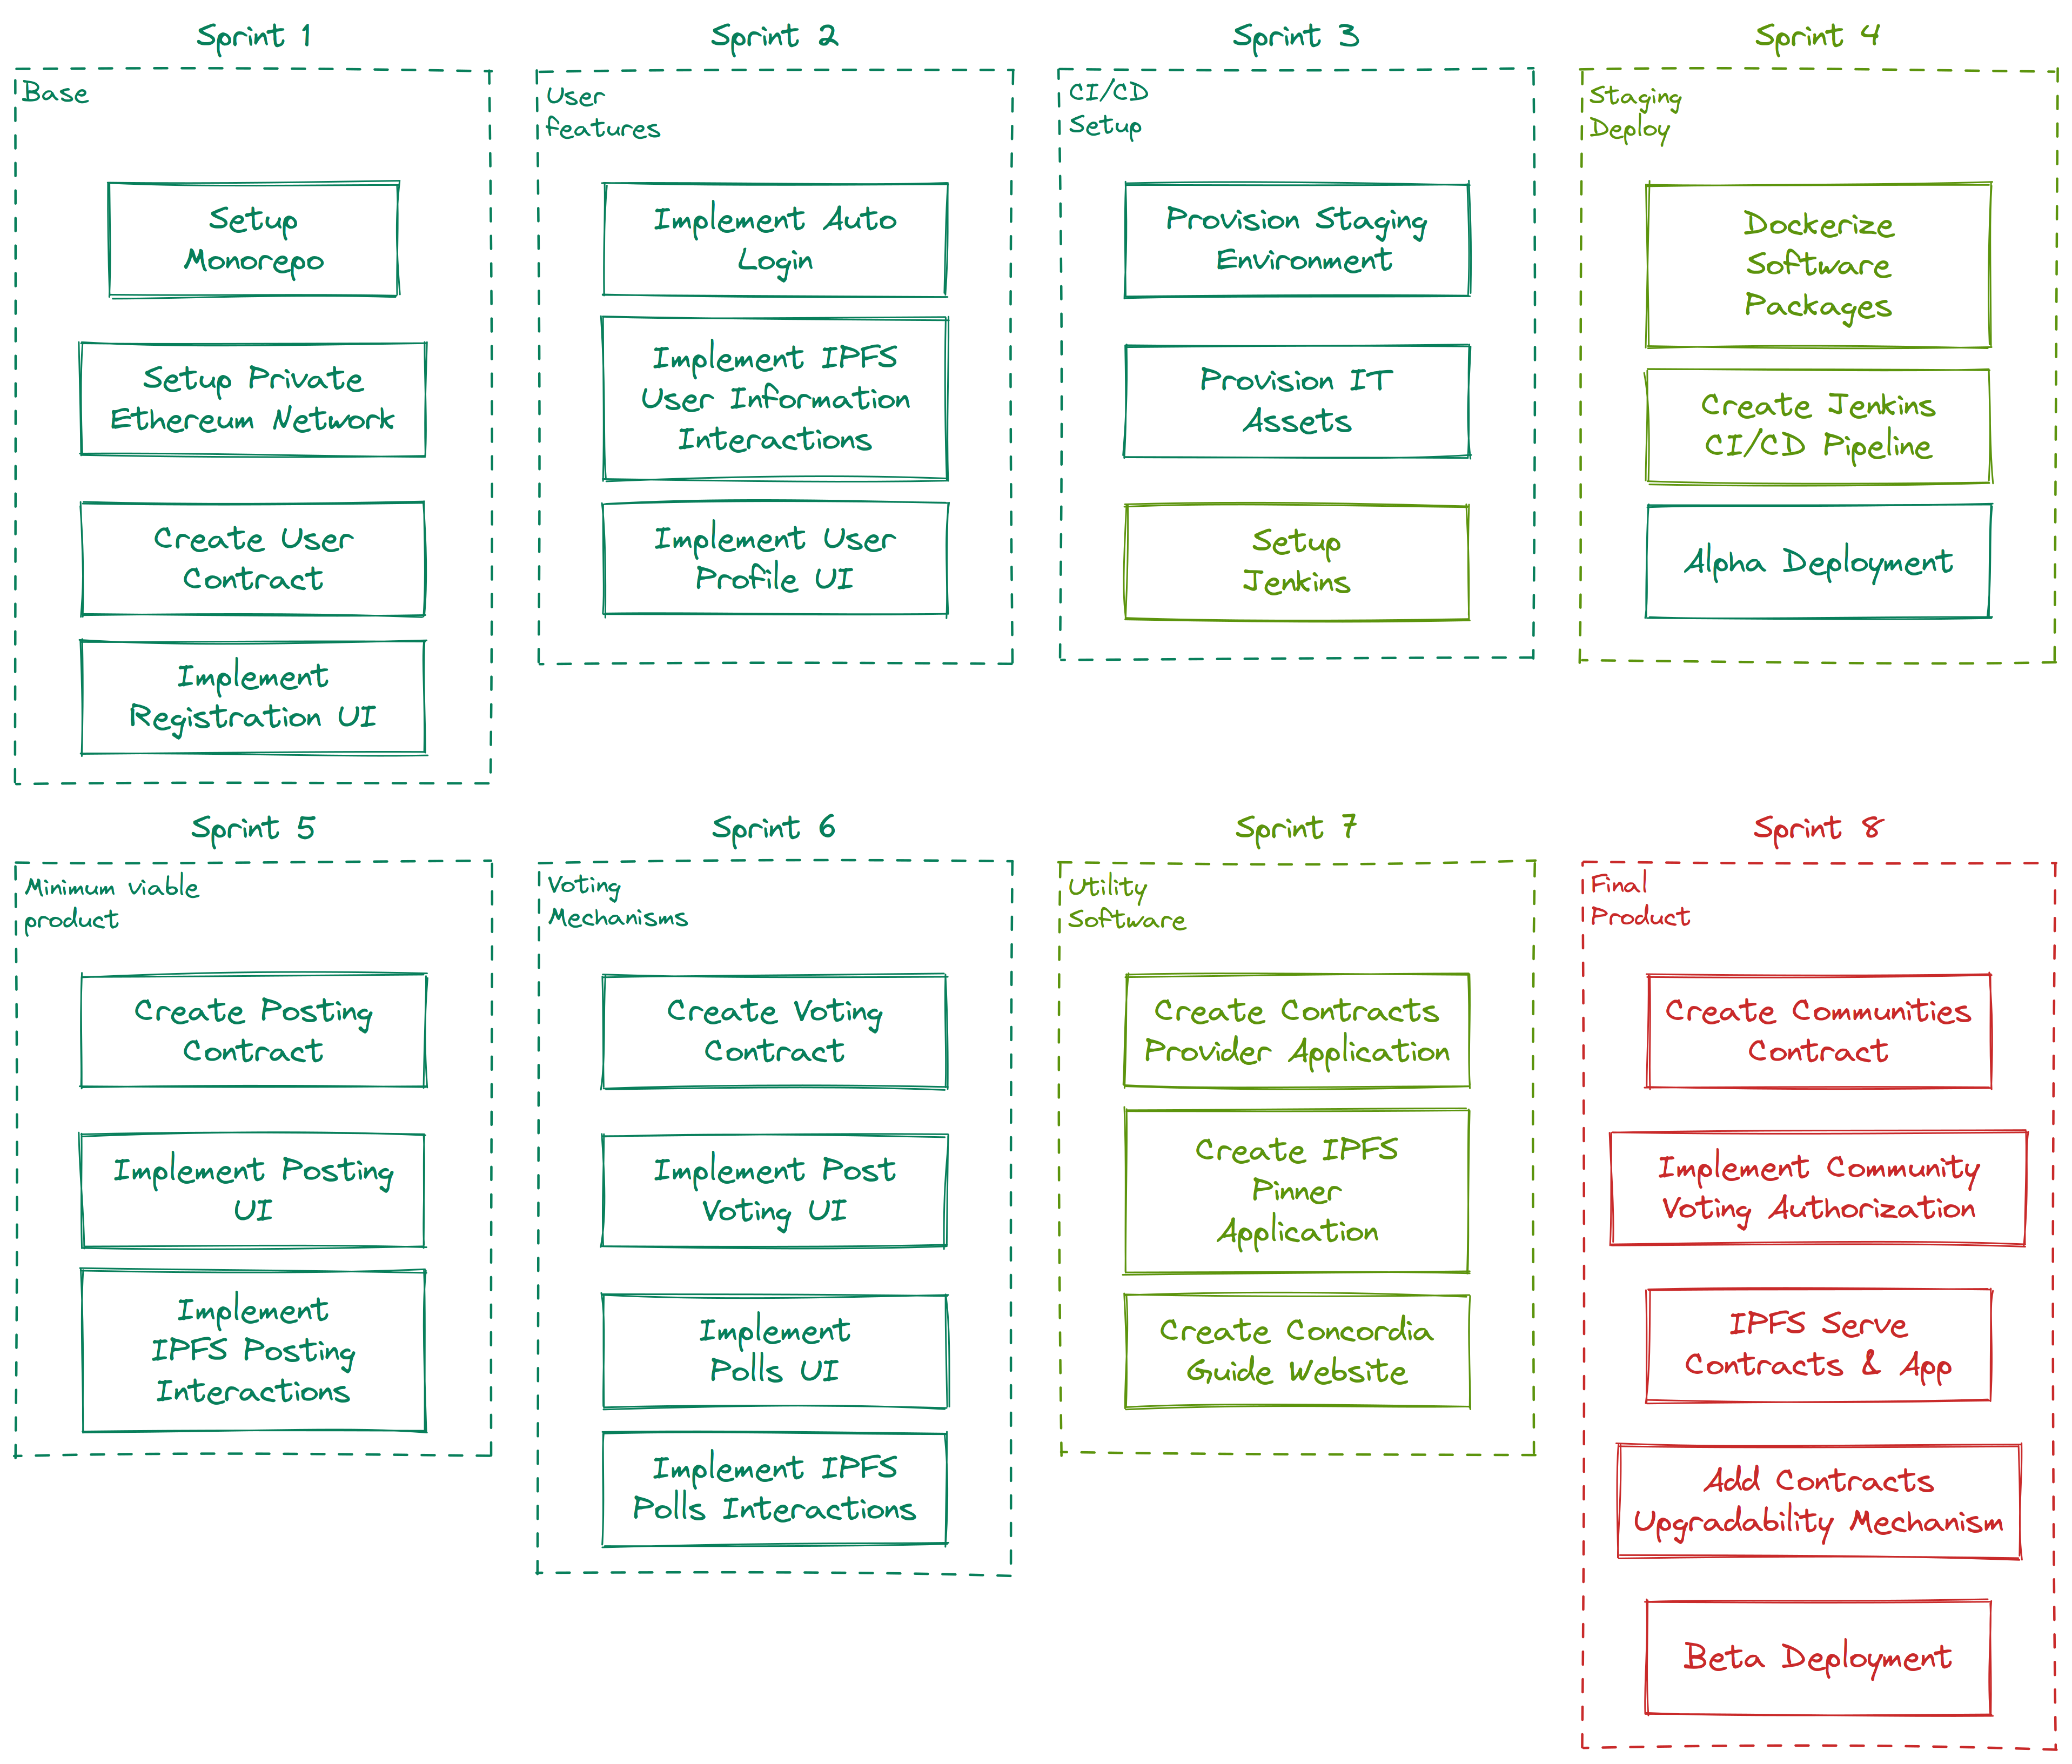
\includegraphics[width=\textwidth]{assets/figures/chapter-4/4.6.design-implementation-differences-sprints.png}
    \caption{Διαχωρισμός σε sprints}
    \label{figure:4.6.design-implementation-differences-sprints}
\end{figure}
